\chapter{Introdução}

A introdução eu devo escrever por último, deve conter a importancia do projeto, devo descrever o problema e a solução: "existe um problema e foi resolvido assim". O final da introdução deve descrever a estrutura dos capitulos dando uma pincelada rapida em cada um.

\chapter{Conceitos}
\section{Arquitetura de Software}
\section{Atributos de Modularidade}
\subsection{Acoplamento}
\subsection{Coesão}

\chapter{Implementação do Extrator}

Neste capítulo deve documentar o que fiz e como fiz, as dificuldades encontradas no processo, etc...

\section{egypt}

egypt é um programa originalmente desenvolvido por Andreas Gustafsson\footnote{http://www.gson.org/egypt} para gerar gráfico de chamada entre funções de programas escrito em C, ele funciona lendo os arquivos intermediários gerados pelo GCC\sigla{GCC}{GNU C Compiler} e converte isto num gráfico de chamada no formato usado pelo Graphviz\footnote{http://www.graphviz.org} um programa de visualização de gráficos.

O egypt é software livre e em Janeiro de 2009 começou a ser restruturado por Antonio A S. Terceiro o qual tem mantido em\footnote{http://github.com/terceiro/egypt}. As principais mudanças sofridas pelo egypt foram \cite{StructuralComplexityEvolution}:

\begin{itemize}
\item Implementação de detecção de uso de variáveis, para identificar que função usa qual variável.
\item Opção para agrupar chamadas e uso de variaveis por módulo, com isto é possível ter uma visão de dependencia entre módulos.
\item Refatoração do script egypt para um design orientado a objetos para permitir diferentes módulos de extração e relatório.
\item Implementação de geração de relatório de métricas.
\end{itemize}

Em sua versão original o egypt necessita que seja executado o GCC nos fontes do projeto que se deseja analisar, com isto o tempo de análise de um de um grande projeto torna-se bastante longo e as vezes inviável.

\section{Doxygen (e a sua API)}

Doxygen\footnote{http://www.doxygen.org} é um sistema de documentação para C, C++, Java, Python e outros. Com ele é possível gerar documentação em HTML, RTF, PostScript, PDF e man pages. Ele extrai a documentação explícita desenvolvida pelo programador dos comentários no código fonte seguindo uma sintaxe própria, mas também pode ser configurado para extrair diretamente dos fontes a hierarquia e colaboração entre as classes. É baseado neste recurso de poder extrair a estrutura do código fonte sem necessitar de documentação explícita que o Doxygen foi escolhido para implementar um extrator para o egypt.

O Doxygen é Software Livre e está disponível sob a GPL \sigla{GPL}{GNU Public License} em \footnote{https://doxygen.svn.sourceforge.net/svnroot/doxygen/trunk}, o código fonte dele vem com o exemplo de uma ferramenta para parsing de código fonte bem próximo as necessidades deste projeto.

\section{Implementação do Extrator usando a API do Doxygen}

O Doxygen apesar de oferecer todos os recursos básicos necessários para analisar um código fonte em C/C++ e extrair o uso de símbolos (funções, varáveis, etc) não faz o trabalho de simplesmente extrair estes dados sem gerar saída em PDF ou RTF por exemplo.

A API do Doxygen fornece uma interface para quem deseja escrever trecho de código fora dos comentários do projeto analisado para um formato específico como Latex ou HTML por exemplo. Seguindo esta interface CodeOutputInterface é possível implementar um parser reaproveitando todo o poder que o Doxygen fornece para análise de código fonte e gerar uma saída da forma desejada.

Neste projeto foi implementado uma ferramenta chamado doxyparse seguindo esta interface onde são definidos parametros para o Doxygen deacordo com as nossas necessidades como por exemplo: analisar o diretorio recursivamente, não gerar saida em Latex ou HTML, extrair tant informação quanto possível do codigo fonte, gerar gráfico de chamada, etc.

Este parser então faz a análise dos fontes de um diretorio passado via linha de comando e extrai destes fontes os simbolos encontrados onde são definidos e onde são usados/chamados. Com isto em mão ele gera uma saída num formato convinente para ser depois analisado pelo extrator implementado no egypt. Exemplo de saída gerado pelo doxyparse:

\begin{verbatim}
module module1.c
   function main in line 5
      uses function callback defined in module3.c
      uses function say_bye defined in module2.c
      uses function say_hello defined in module2.c
      uses variable variable defined in module3.c
\end{verbatim}

Com a saída gerada pelo doxyparse em mãos o egypt precisa agora de um extrator que entenda estes dados e armazene as informações encontradas para então depois gerar a saída para o Graphviz gerar o gráfico ou para gerar as métricas implementadas no egypt. Como o egypt já tem uma infraestrutura para possibilitar novos extratores não foi difícil criar um novo, o egypt possui uma classe chamada Extractor que representa extrator baseado nos arquivos intermediários do GCC, este classe foi transformada numa implementação de extrator genérica contendo apenas uma interface para cada extrator especifico implmentar e foi criado inicialmente 2 estratores, o GCC baseado no código já existente e o Doxyparse um novo extrator que usa como entrada os dados gerados pelo doxyparse baseado no Doxygen.

\begin{figure}[h]
\center
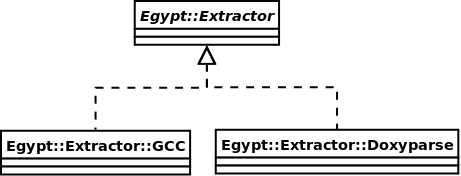
\includegraphics[scale=0.5]{imagens/egypt-diagram-extractor}
\label{egypt-diagram-extractor}
\caption{diagrama da hierarquia de classes do extrator do egypt}
\end{figure}

\chapter{Avaliação}
\section{Procedimento}
\section{Resultados}

Nos resultados eu posso comparar o que consegui com a nova ferramenta comparado ao modo antigo do egypt extrair informacoes.

%\begin{figure}[h]
%\center
%\subfigure[ristretto-0.0.1-doxyparse][Egypt::Extrator::Doxyparse]{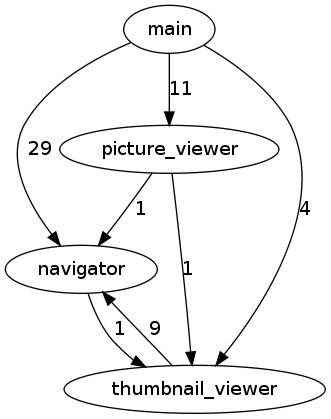
\includegraphics[scale=0.5]{imagens/ristretto-0_0_1-doxyparse}}
%\qquad
%\subfigure[ristretto-0.0.1-gcc][Egypt::Extrator::GCC]{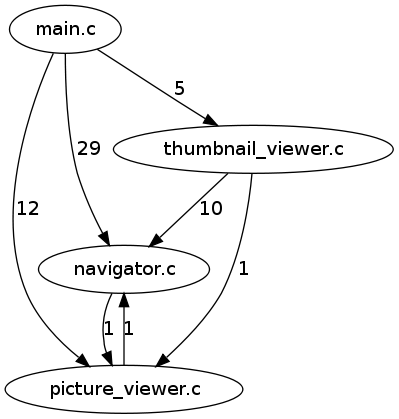
\includegraphics[scale=0.5]{imagens/ristretto-0_0_1-gcc}}
%\caption{gráfico de chamada entre módulos do {\bf Ristretto 0.0.1} gerado pelo Egypt}
%\end{figure}
%
%\begin{figure}[h]
%\center
%\subfigure[ristretto-0.0.11-doxyparse][Egypt::Extrator::Doxyparse]{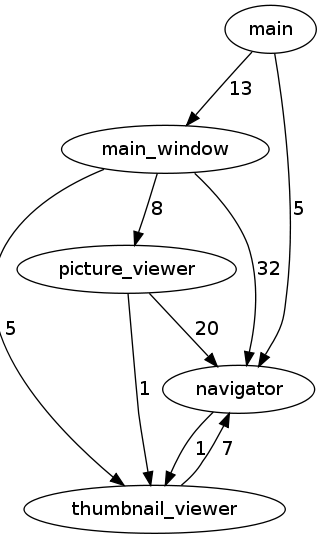
\includegraphics[scale=0.5]{imagens/ristretto-0_0_11-doxyparse}}
%\qquad
%\subfigure[ristretto-0.0.11-gcc][Egypt::Extrator::GCC]{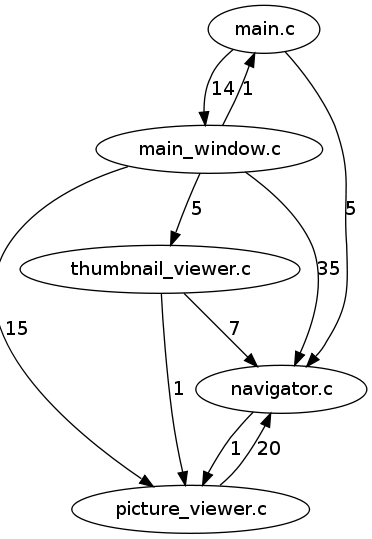
\includegraphics[scale=0.5]{imagens/ristretto-0_0_11-gcc}}
%\caption{gráfico de chamada entre módulos do {\bf Ristretto 0.0.11} gerado pelo Egypt}
%\end{figure}
%
%\begin{figure}[h]
%\center
%\subfigure[ristretto-0.0.21-doxyparse][Egypt::Extrator::Doxyparse]{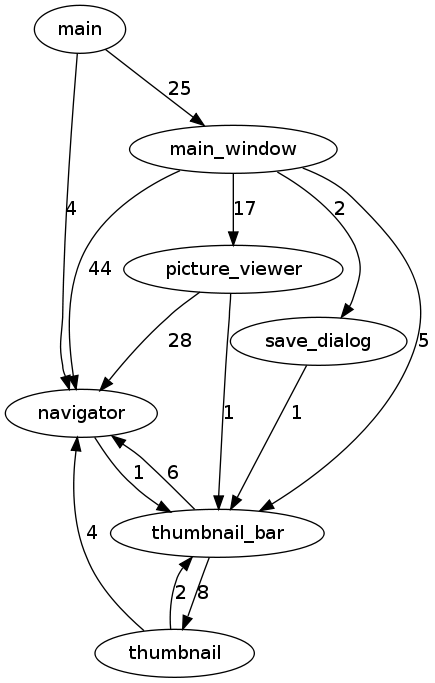
\includegraphics[scale=0.5]{imagens/ristretto-0_0_21-doxyparse}}
%\qquad
%\subfigure[ristretto-0.0.21-gcc][Egypt::Extrator::GCC]{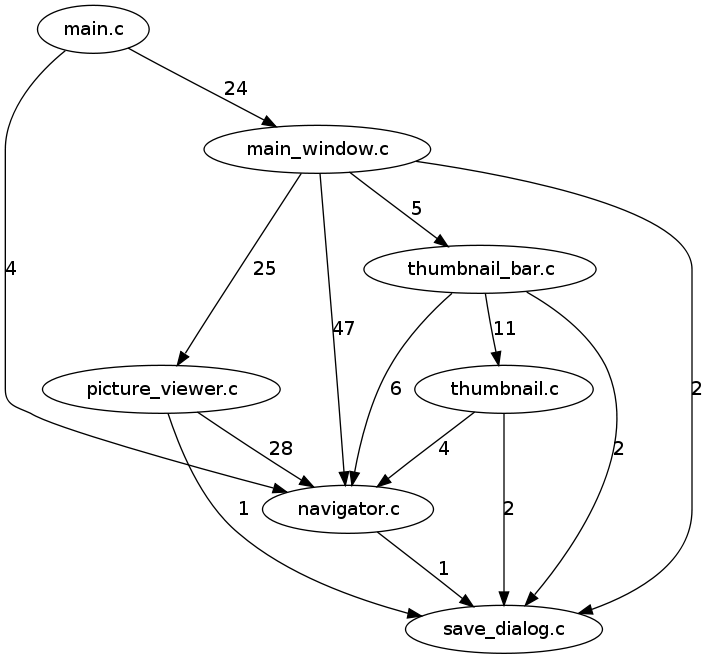
\includegraphics[scale=0.5]{imagens/ristretto-0_0_21-gcc}}
%\caption{gráfico de chamada entre módulos do {\bf Ristretto 0.0.21} gerado pelo Egypt}
%\end{figure}

\section{Discussão}

\chapter{Conclusão}

A conclusão eu devo escrever por último, deve conter algo assim: "Este trabalho tinha objetivo tal e atingiu tal objetivo". Deve ter referencia de como foi feito e se os resultados foram bons, medios, satisfatorios, ruins, etc. E ao final deve ter trabalhos futuros que eu tenha interesse ou não de fazer.

Trabalhos futuros: verificar Natural Docs, semelhando ao Doxygen implementado em Perl e suporta outras linguagens.
